\chapterfont{\huge\color{LightBlue}}  % sets colour of chapter
\sectionfont{\color{LightBlue}}  % sets colour of sections
\subsectionfont{\color{LightBlue}}  % sets colour of subsections

\renewcommand\pcolor{LightBlue}
\renewcommand{\headrule}{\hbox to\headwidth{%
		\color{LightBlue}\leaders\hrule height \headrulewidth\hfill}} % color of title
\fancyfoot[LE,RO]{\thepage}



\cleardoublepage
\makeatletter
\let\savedchap\@makechapterhead
\def\@makechapterhead{\vspace*{-3cm}\savedchap}
\chapter[The genetic architecture of molecular traits]{The genetic architecture of molecular traits}
\chaptermark{}
\let\@makechapterhead\savedchap
\makeatletter
\label{chap:chapter2-genetic-architecture}

\hfill \underline{Current Opinion in Systems Biology.} 2017 Feb 16; Volume 1: p25-31.

\hfill DOI: \href{https://doi.org/10.1016/j.coisb.2017.01.002}{j.coisb.2017.01.002}
\\
\\
Annique Claringbould\textsuperscript{*}, Niek de Klein\textsuperscript{*}, Lude Franke\textsuperscript
\\
\\
* These authors contributed equally to this work.

\newpage

{ \Large \leftwatermark{
		\put(-50,-66.5){ 1 }
		\put(-97.5,-101){
\includegraphics[scale=0.8]{img/thumbindex/thumbindex_LightBlue.eps}}  
		\put(-50,-91.5){ {\color{white} 2 }}
		\put(-50,-116.5){ 3 }
		\put(-50,-141.5){ 4 }
		\put(-50,-166.5){ 5 }
		\put(-50,-191.5){ 6 }
	} \rightwatermark{
		\put(388,-66.5){ 1 }
		\put(380,-101){
\includegraphics[scale=0.8]{img/thumbindex/thumbindex_LightBlue.eps}}  
		\put(388,-91.5){ {\color{white} 2 }}
		\put(388,-116.5){ 3 }
		\put(388,-141.5){ 4 }
		\put(388,-166.5){ 5 }
		\put(388,-191.5){ 6 }
}}

\section*{Abstract}

Most diseases have both an environmental and genetic component. Although many diseases are strongly heritable, individual genetic variants typically confer only a small effect on disease, and thus these diseases are strongly polygenic. Paradoxically, molecular traits, such as gene expression, methylation, protein or metabolite levels, typically have a lower heritability, but sometimes individual genetic variants show much higher effect sizes on these traits. In this review we discuss the genetic architecture of these molecular traits, and contrast this to the genetic architecture of complex diseases, and provide explanations why strong effects of individual genetic variants on molecular traits do not necessarily need to translate into increased risk of disease.
\\
\\
\begin{figure}[h!]
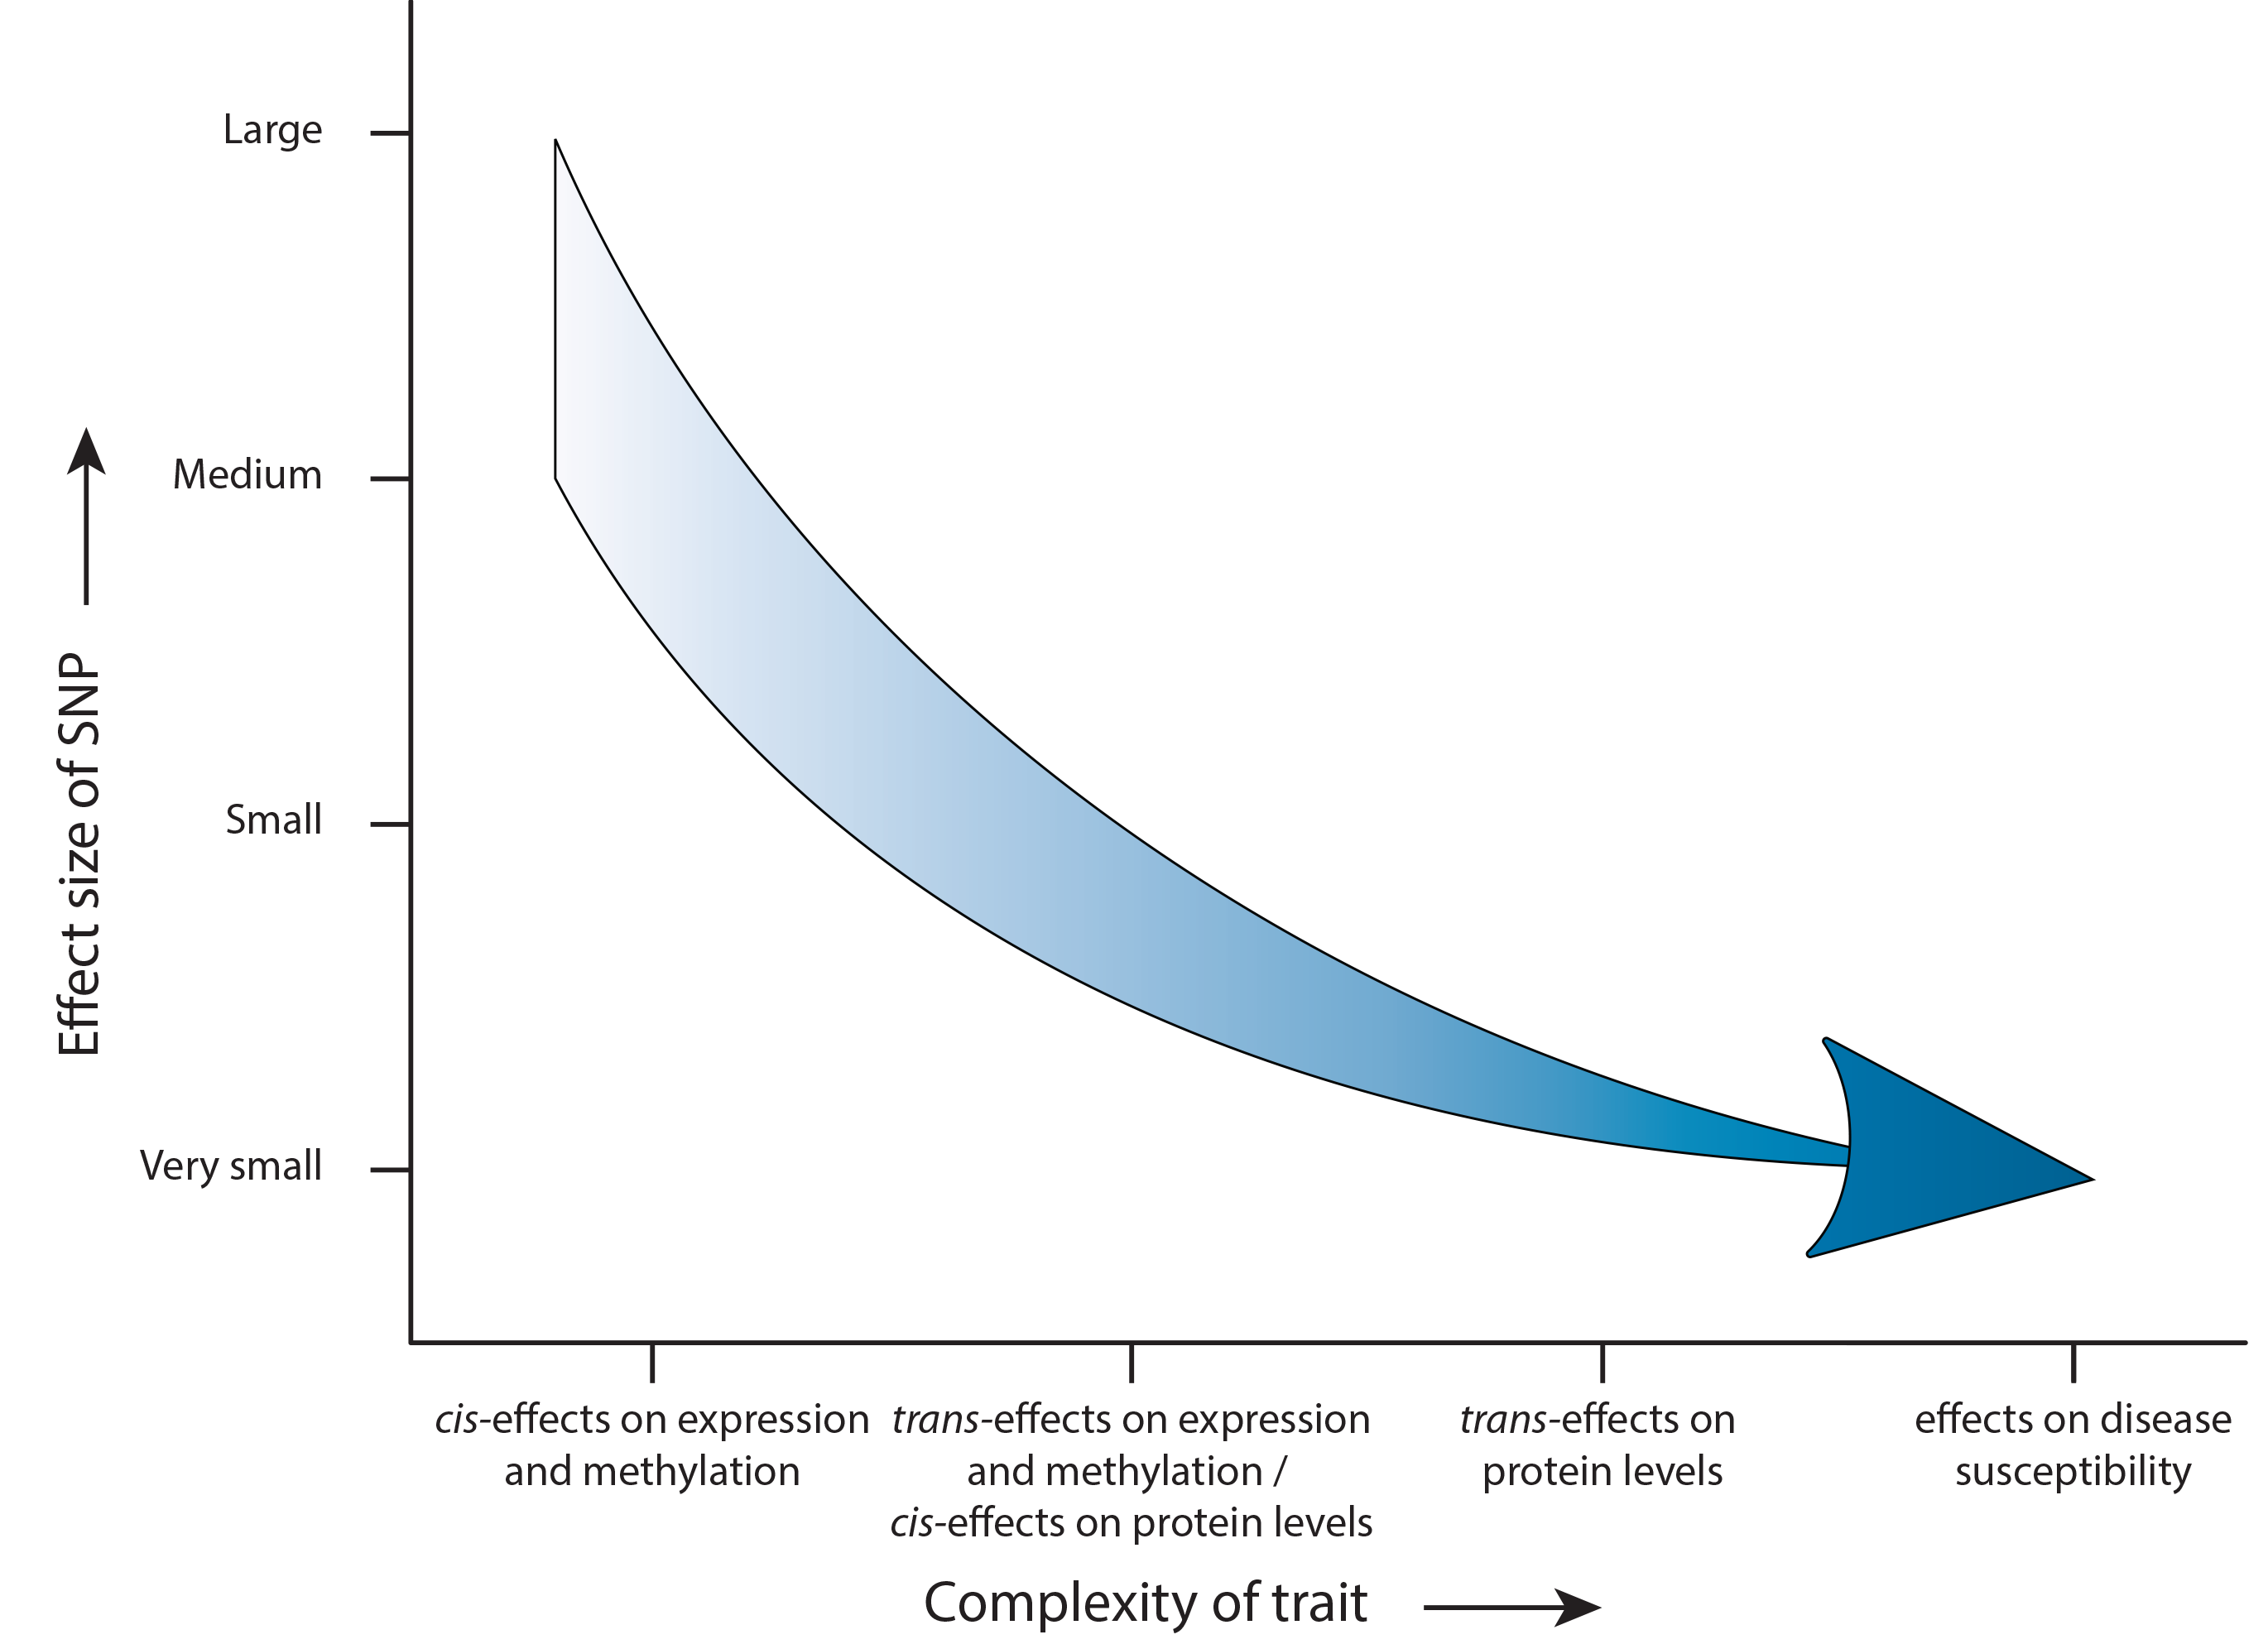
\includegraphics[scale=0.1]{chapters/chapter2-genetic-architecture/img/AbstractFigureCorrectSizeWhite}
\caption{Graphical abstract}
\end{figure}


\Needspace{10\baselineskip}
\section{Introduction}

Since most diseases, phenotypes, and molecular traits are heritable, their genetic architecture is a long-standing question. Are most phenotypes caused by a limited number of large effect variants, or are they due to many variants that each have a small effect? In this review, we compare detected effect size and allele frequencies of associated variants from genome-wide association studies (GWAS) on complex traits and diseases with results from expression- and methylation quantitative trait locus (eQTL and meQTL) studies.

\Needspace{10\baselineskip}
\section{Genetic architecture of common disease: few large effects}
Over the last few years, GWAS have shown that associated variants typically only explain a small proportion of the disease variation seen in the majority of common diseases, despite a few examples of common variants with a large effect being found for immune-related traits, particularly in the HLA-region \cite{dalyHLAB5701Genotype2009}. Currently, variants with an odds ratio (OR) $>$ 10 are considered ‘highly unusual’ \cite{mccarthyGenomewideAssociationStudies2008}. These observations led to an extensive debate about the genetic architecture of complex diseases \cite{mccarthyGenomewideAssociationStudies2008,hansenEvolutionGeneticArchitecture2006,devlinGeneticArchitectureAutism2012,lohContrastingGeneticArchitectures2015,fuchsbergerGeneticArchitectureType2016}, including issues like the number, frequency and effect size of associated genetic variants, as well as the degree of shared genetic background with other traits \cite{mackayGeneticArchitectureQuantitative2001}. For complex diseases the architecture is by no means uniform: the number of genes and their effect sizes differ widely \cite{lohContrastingGeneticArchitectures2015,fuchsbergerGeneticArchitectureType2016,HiddenComplexityMendelian,rheenenGenomewideAssociationAnalyses2016}. However, there is evidence for a shared genetic basis among many diseases \cite{zhernakovaDetectingSharedPathogenesis2009,pickrellDetectionInterpretationShared2016,shiContrastingGeneticArchitecture2016}, and the genetic architecture of most complex disease seems to be highly polygenic.

A much cited interpretation of the overall genetic architecture of diseases places genetic variants in five different groups, based on their allele frequency and effect size or penetrance (\textbf{Figure \ref{architecture_fig1}A}, adapted from \cite{mccarthyGenomewideAssociationStudies2008,manolioFindingMissingHeritability2009}). In this representation, complex diseases are characterized by many common genetic variants with small effect sizes, whereas Mendelian diseases are caused by rare variants with large effects. Subsequently, methods were developed that can infer the variance explained by using all directly genotyped SNPs, including those that do not attain genome-wide significance. For complex phenotypes such as height it was established that a considerable proportion of the heritability could be explained by common SNPs, suggesting a highly polygenic genetic architecture \cite{yangCommonSNPsExplain2010}.

\begin{figure}[H]
	\includegraphics[scale=0.3]{chapters/chapter2-genetic-architecture/img/Figure1.png}
	\caption{\footnotesize \textbf{(A)} Proposed genetic architecture of diseases, adapted from Refs. 2, 13. \textbf{(B)} Minor allele frequency (MAF) set out against odds ratio (OR) of genome-wide significant GWAS SNPs. The data is downloaded from the GWAS catalog (Supplementary Note 1). Histograms on the right and at the top indicate the frequency distribution of the SNPs, the dot size indicates the total sample size of the GWAS, and the color represents the year of publication. Rare and intermediate frequency variants (MAF < 0.1) have a higher OR on average. \textbf{(C)} MAF against variance explained (R2) of \textit{cis} expression quantitative trait locus (eQTL) SNPs. Light blue SNPs are from the GEUVADIS consortium (N = 373), dark blue SNPs from the BIOS consortium (N = 2116) (Supplementary Note 2). The plots on the top and right of the figure illustrate the density distribution of SNPs from both cohorts. Despite different sample sizes, the distribution of the \textit{cis} eQTL SNPs is similar for both cohorts. \textbf{(D)} MAF against variance explained (R2) of \textit{cis} and \textit{trans} methylation quantitative trait locus (eQTL) SNPs. Dark blue SNPs are \textit{cis} meQTLs and light blue SNPs are \textit{trans} meQTLs (Supplementary Note 3). Histograms on the right and at the top indicate the frequency distribution of the SNPs. Common SNPs often have large effect sizes, and \textit{trans} effects explain much less methylation variation on average.}
	\label{architecture_fig1}
\end{figure}

Indeed, an inventory of the binary traits in the GWAS Catalog (v1.01, r2016-06-12, p $<$ 5x10-8, Supplementary Note 1) reveals that most identified SNPs are common (minor allele frequency (MAF) $>$ 0.1) and have small effect sizes (OR between 1.0 and 1.2, figure \ref{architecture_fig1}B). The expectation was that by increasing sample sizes, GWAS would also allow for finding the intermediate frequency variants (0.005 $<$ MAF $<$ 0.1) with larger effects on disease. However, even very large studies have not yet been able to identify many of these hypothesized large effect variants \cite{fuchsbergerGeneticArchitectureType2016} (\textbf{Figure \ref{architecture_fig1}B}), while recent studies show that they can be more successfully detected by whole-genome sequencing \cite{del-aguilaAlzheimerDiseaseRare2015,walterUK10KProjectIdentifies2015}.

\Needspace{10\baselineskip}
\section{Genetic architecture of molecular traits}
Surprisingly, the genetic architecture of complex phenotypic (disease) traits differs substantially from the genetic architecture of molecular traits such as gene expression, methylation, or protein levels. Although the genetic architecture of molecular traits can also be polygenic, a single SNP can often explain a considerable part of the heritability compared to disease phenotypes, whereas the heritability of gene expression, methylation or protein levels is typically lower than complex diseases \cite{wrightHeritabilityGenomicsGene2014,poldermanMetaanalysisHeritabilityHuman2015}. 

\Needspace{10\baselineskip}
\section{Large effect-sizes of SNPs affecting molecular traits}
Genetic variation influences the risk of developing a complex disease through several molecular traits such as gene expression \cite{emilssonGeneticsGeneExpression2008} and methylation \cite{conerlyInsightsRoleDNA2010}. Investigating eQTLs \cite{pickrellUnderstandingMechanismsUnderlying2010,lappalainenTranscriptomeGenomeSequencing2013,westraSystematicIdentificationTrans2013,zhernakovaIdentificationContextdependentExpression2017,gibsonExpressionQuantitativeTrait2015} and allele-specific expression (ASE) \cite{deelenCallingGenotypesPublic2015,pirinenAssessingAllelespecificExpression2015,rivasEffectPredictedProteintruncating2015,castelToolsBestPractices2015} can characterize the effect of common and rare genetic variants, respectively, on gene expression. Similarly, intermediate frequency and common SNPs that affect methylation levels at CpG sites can be detected by meQTL mapping \cite{bonderDiseaseVariantsAlter2017}.

Analogous to the genetic architecture of common diseases presented in \textbf{Figure \ref{architecture_fig1}B}, the genetic architecture of gene expression and methylation may be represented by plotting the allele frequency of QTLs against their effect size (\textbf{Figure \ref{architecture_fig1}C} and \textbf{1D}, \textbf{Supplementary Note 2}). We first compared the proportion of variance explained for \textit{cis}-eQTLs identified in RNA-seq data in blood (BIOS consortium, N=2,116, only SNPs tested with MAF $>$ 0.05) \cite{zhernakovaIdentificationContextdependentExpression2017} and in Epstein-Barr virus-transformed lymphoblastoid cell lines (GEUVADIS consortium, N=373, only SNPs tested with MAF $>$ 0.05) \cite{lappalainenTranscriptomeGenomeSequencing2013}. Comparing the two cohorts indicates that sample size has an impact on the number of identified eQTL SNPs, but not on their effect size (\textbf{Figure \ref{architecture_fig1}C}). 

Notably, the effects of many eQTLs and meQTLs are large, especially compared to the degree of heritability of a disease explained by GWAS: some eQTLs explain as much as 80\% of the variation at transcript level (\textbf{Figure \ref{architecture_fig1}C}) and many \textit{cis}-meQTLs explain over 70\% of the methylation level variation (\textbf{Figure \ref{architecture_fig1}D}). While common GWAS SNPs only rarely have a large effect on the phenotype, the impact of common SNPs on molecular traits can thus be much greater. 
Another observation is that the minor allele frequency distribution of disease variants (\textbf{Figure \ref{architecture_fig1}B}) is different from the MAF distribution of both eQTLs and meQTLs (\textbf{Figure \ref{architecture_fig1}C} and \textbf{1D}): molecular traits are influenced by variants with on average a lower MAF, as compared to complex traits for which the average MAF is higher.

\Needspace{10\baselineskip}
\section{Many independent SNPs affecting the same molecular trait}
While for many complex diseases many independent associations have so-far been found, the number of independent associations for molecular traits has been studied less well. Conditional analyses (i.e. correction for primary \textit{cis}-eQTLs) can be performed to ascertain whether secondary signals can be identified. Zhernakova et al. (2015) recently performed such an analysis and observed that more than half of the transcripts are governed by more than one \textit{cis}-eQTL effect, suggesting that the genetic architecture of gene expression regulation for most genes is polygenic, similar to complex diseases.

\Needspace{10\baselineskip}
\section{Local and distal effects}
However, these conditional analyses have so-far only identified multiple independent SNPs that are working in \textit{cis}: SNPs most often affect nearby molecular traits in \textit{cis} through mechanisms such as transcription factor binding disruption in regulatory regions or promotor disruption within transcription start sites \cite{brownIntegrativeModelingEQTLs2013}. To identify genetic variants that are distantly located, \textit{trans}-QTL mapping can be conducted. Those \textit{trans} effects are hypothesized to be mediated by multiple \textit{cis} effects and complex downstream regulation on a molecular trait \cite{westraSystematicIdentificationTrans2013,wongInterplayCisTrans2017}, and are identified less frequently (\textbf{Figure \ref{architecture_fig2}}), due to severe multiple-testing issues when comparing millions of genetic variants with tens of thousands of molecular traits. So-far the largest QTL studies have observed a \textit{trans}-acting proportion of 4.5\% \cite{westraSystematicIdentificationTrans2013} and 2.4\% \cite{wrightHeritabilityGenomicsGene2014} of total eQTLs, and 3.6\% \cite{bonderDiseaseVariantsAlter2017} and 6.5\% for meQTLs \cite{gauntSystematicIdentificationGenetic2016}. With increasing sample-sizes these estimates will likely go up in the near future, since it has been estimated that \textit{cis}-effects explain only 23\% of the total heritability of gene expression level regulation \cite{wrightHeritabilityGenomicsGene2014}, thus suggesting that distal effects strongly outnumber local effects. However, for both eQTLs and meQTLs, the \textit{cis} effect sizes are on average several times higher than the \textit{trans} effects (\textbf{Figure \ref{architecture_fig1}D} and \ref{architecture_fig3}A), which is likely due to additional regulation layers between the \textit{cis} effect and the \textit{trans} effect \cite{albertRoleRegulatoryVariation2015}. 

\begin{figure}[H]
	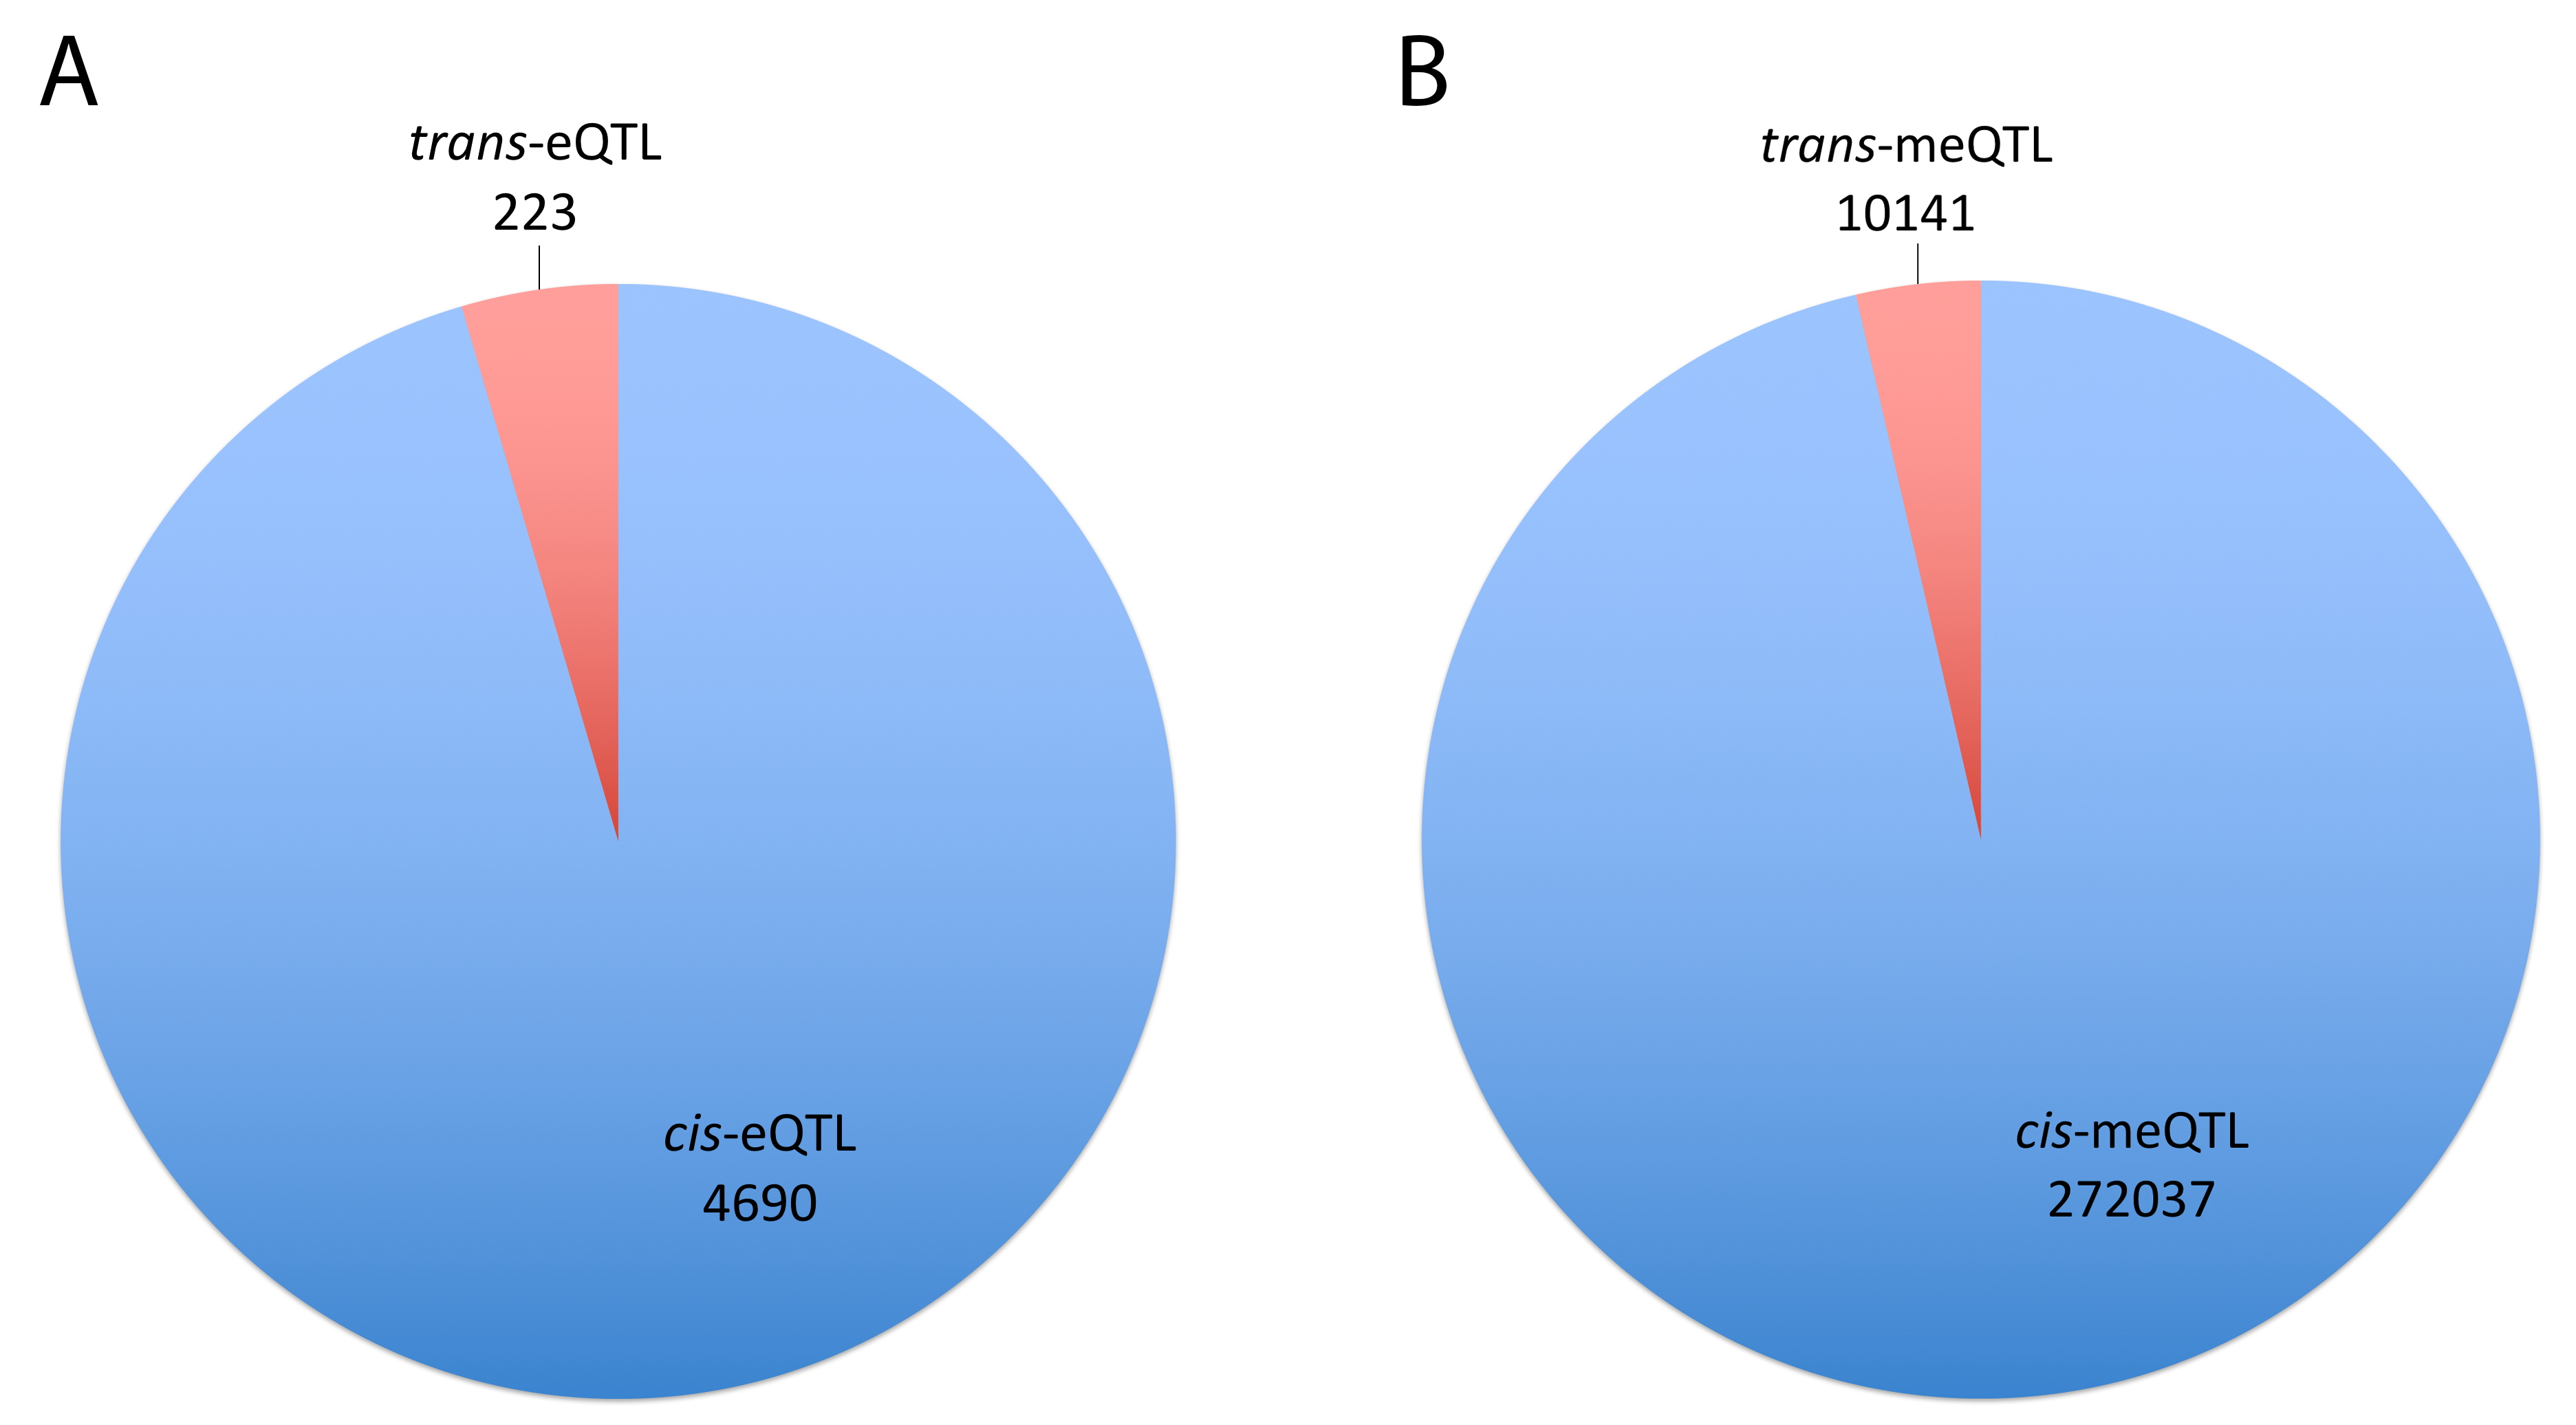
\includegraphics[width=\textwidth]{chapters/chapter2-genetic-architecture/img/Figure2.png}
	\caption{\textbf{(A)}, \textbf{(B)} Pie charts comparing the number of observed eQTLs \textbf{(A)} and meQTLs \textbf{(B)} based on Refs. \cite{zhernakovaIdentificationContextdependentExpression2017,wongInterplayCisTrans2017}. Blue indicates \textit{cis} effects, red are the \textit{trans} effects.}
	\label{architecture_fig2}
\end{figure}



With the current sample-sizes, the percentage of tested genes with a significant QTL is higher for \textit{cis} than for \textit{trans} (\textbf{Figure \ref{architecture_fig3}A}). This will undoubtedly change when sample-sizes increase further. However, what can be concluded now is that the proportion of CpG sites that show \textit{trans}-meQTL effects is lower than the proportion of genes with a \textit{trans}-eQTL effect. When accounting for the different numbers of samples in \textit{trans}-eQTL and \textit{trans}-meQTL studies this pictue does not change. This indicates that gene expression levels are more polygenic than methylation levels. 

\begin{figure}[H]
	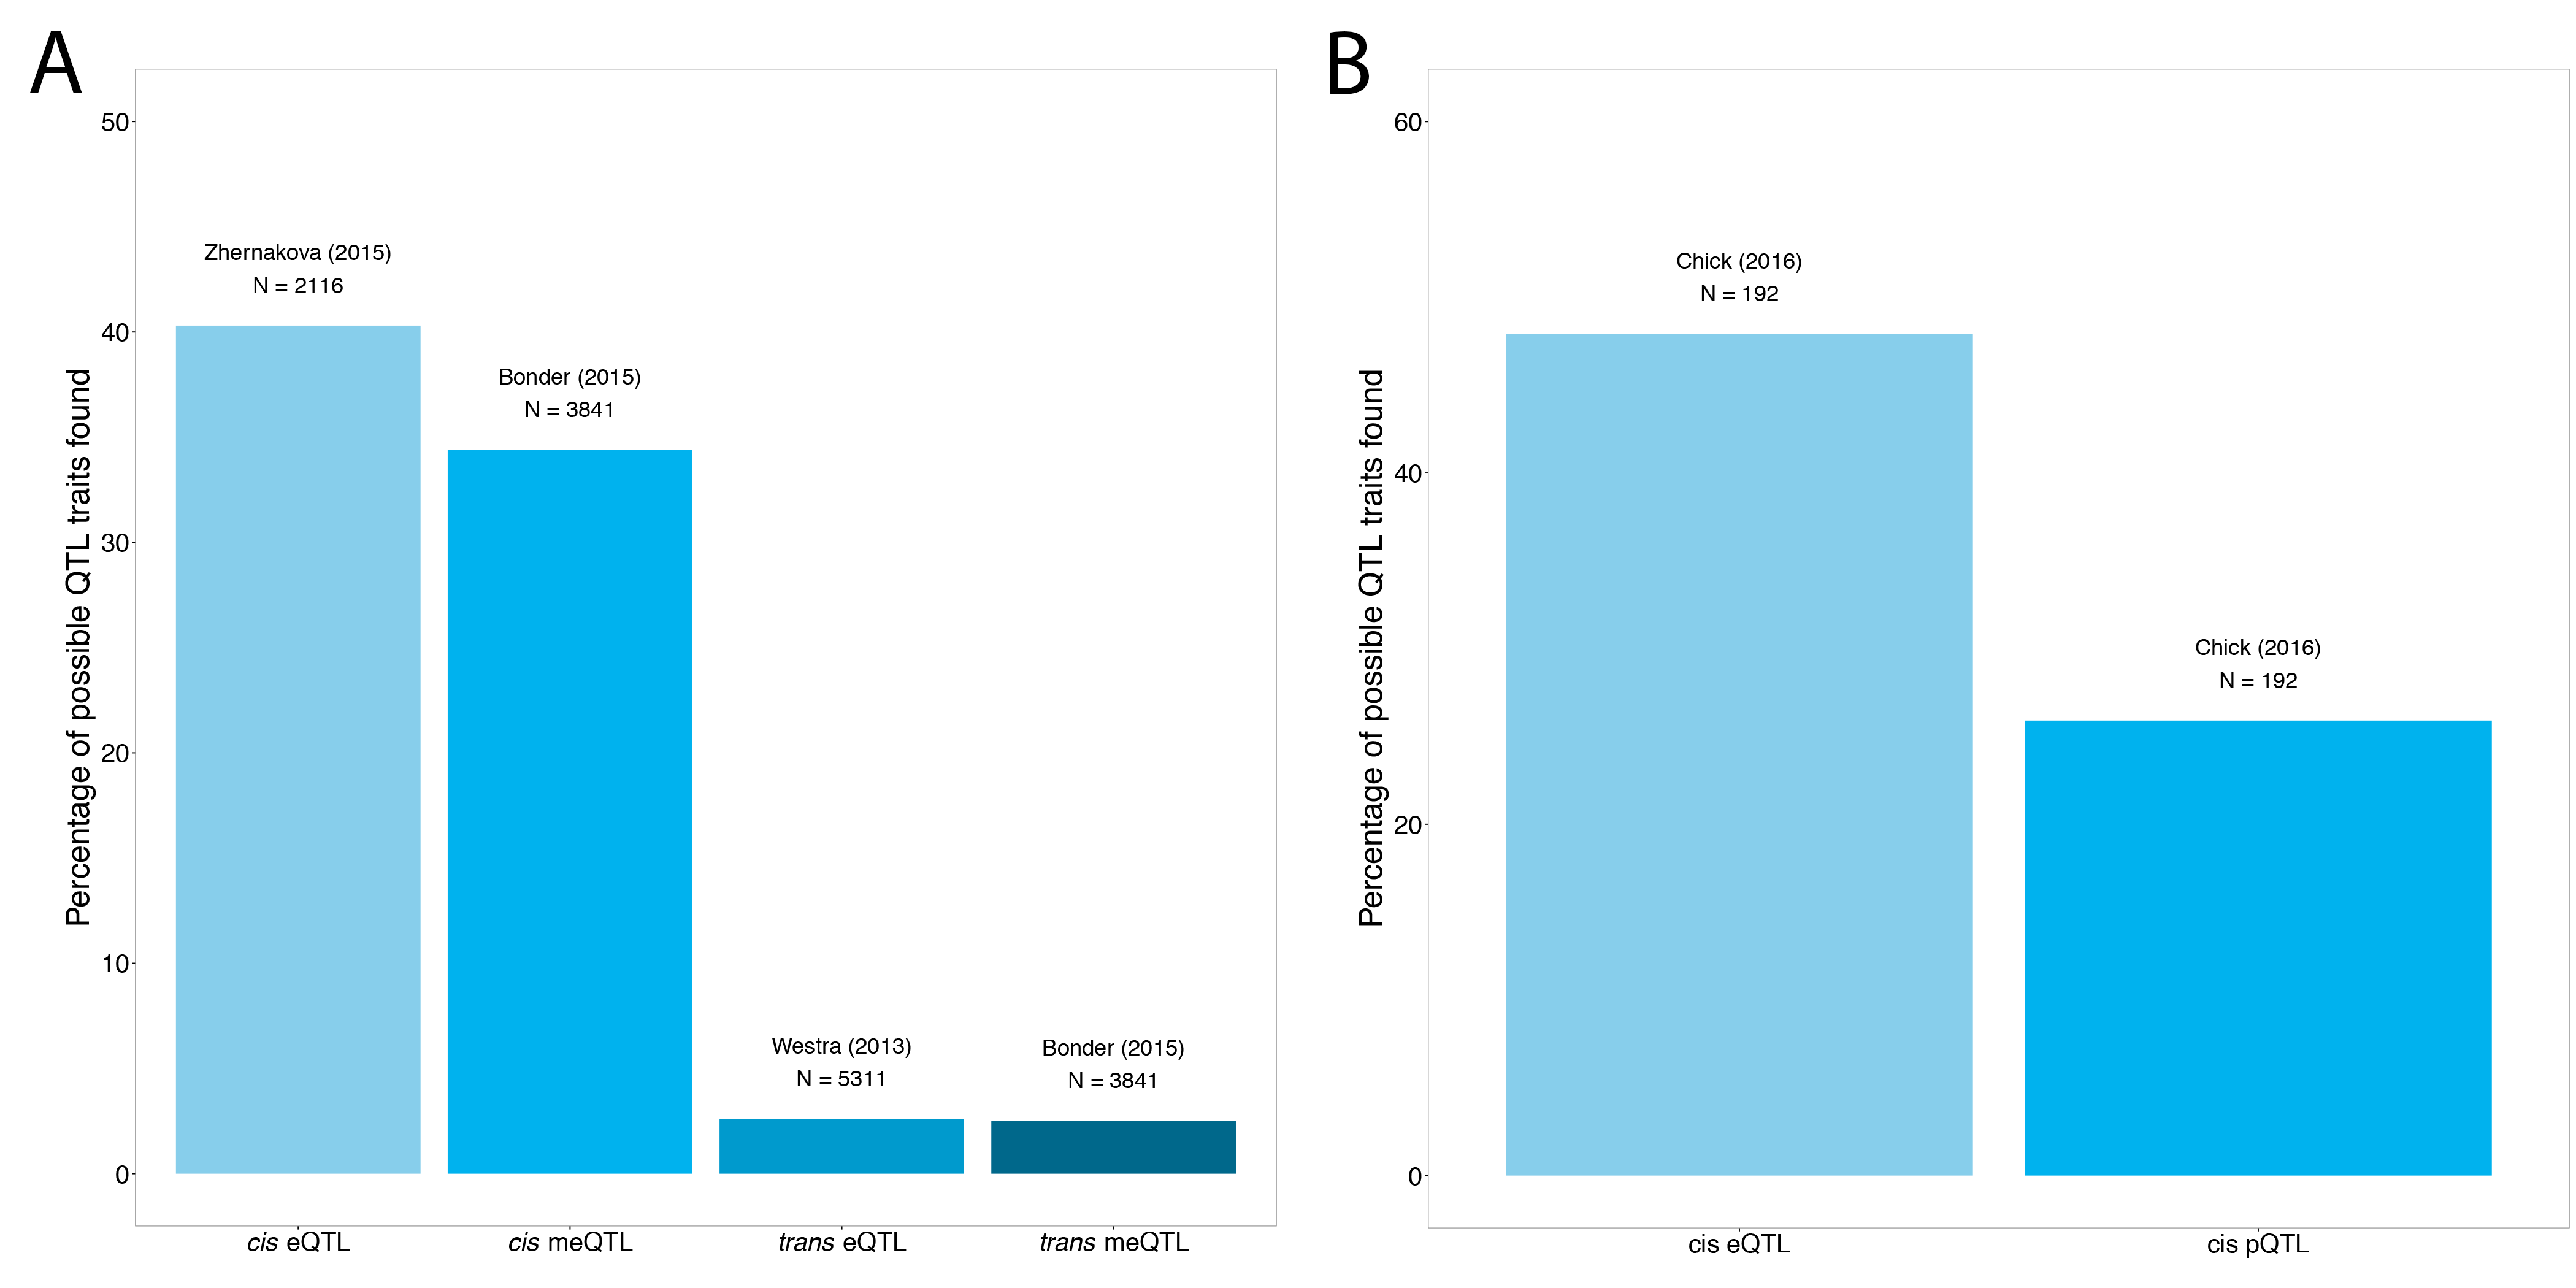
\includegraphics[width=\textwidth]{chapters/chapter2-genetic-architecture/img/Figure3.png}
	\caption{\textbf{(A)} Percentage of total measured SNPs detected as \textit{cis} eQTL, \textit{cis} meQTL, \textit{trans} eQTL and \textit{trans} meQTL SNPs, based on Refs. \cite{zhernakovaIdentificationContextdependentExpression2017,gibsonExpressionQuantitativeTrait2015,wongInterplayCisTrans2017}. Cis effects are identified for a much larger percentage of SNPs compared to \textit{trans} effects. \textbf{(B)} Percentage of total measured SNPs detected as \textit{cis} eQTL, and \textit{cis} protein QTL (pQTL) SNPs in mice, based on Ref. \cite{GenomeWideMetabolicQTL}. For the same mice and the same number of transcripts and proteins, eQTLs are more often detected than pQTLs.}
	\label{architecture_fig3}
\end{figure}

\Needspace{10\baselineskip}
\section{Cell-type and context-specificity of QTLs}
It should be noted, however, that the effects of genetic variants on molecular traits are highly variable: it is now clear that the effects of genetic variation on gene expression levels can depend strongly on cell type, tissue type, and context, such as stimulations by pathogens \cite{fuUnravelingRegulatoryMechanisms2012,gat-viksDecipheringMolecularCircuits2013,fairfaxInnateImmuneActivity2014,leeCommonGeneticVariants2014,meleHumanTranscriptomeTissues2015}. Indeed, blood \textit{cis}-eQTLs are often inconsistent in other tissues: blood QTLs may be absent in a different tissue, they may have a different effect size, or even show an opposite allelic effect \cite{fuUnravelingRegulatoryMechanisms2012}. This is even more pronounced for \textit{trans}-eQTLs: some \textit{trans}-eQTLs can only be replicated in a specific cell type \cite{westraSystematicIdentificationTrans2013}. Tissue-dependent eQTL effects are enriched in SNPs associated with complex traits \cite{fuUnravelingRegulatoryMechanisms2012}, while the cell-type specific effects identified in the HLA region \cite{fairfaxGeneticsGeneExpression2012} are just one example of how tissue specificity can influence the risk of developing the disease. Surprisingly, \textit{trans}-meQTLs are much more stable across cell types \cite{gutierrez-arcelusTissueSpecificEffectsGenetic2015}: it has been shown that the far majority of whole blood \textit{trans}-meQTLs replicate in lymphocytes \cite{bonderDiseaseVariantsAlter2017}, suggesting that meQTLs are generally very stable. It should be noted though, exceptions exist: there are tissue-specific methylation patterns \cite{lokkDNAMethylomeProfiling2014} and \textit{cis}-meQTLs have been found whose CpG levels show correlations with expression levels of tissue-specific alternatively spliced exons \cite{gutierrez-arcelusTissueSpecificEffectsGenetic2015}.

\Needspace{10\baselineskip}
\section{Genetic architecture of other protein and metabolite levels}
Eventually changes in methylation and particularly gene expression levels due to genetic variation should show downstream consequences. Since gene expression levels are not a direct proxy for protein levels \cite{partsHeritabilityGeneticBasis2014,liuInterdependenceTranscriptProtein2016}, protein quantitative trait loci (pQTLs) can give a more accurate measurement of the effect of SNPs on protein abundance. Interestingly, not all pQTLs overlap with eQTLs, suggesting that multiple mechanisms regulate protein levels \cite{wuVariationGeneticControl2013,liuQuantitativeVariability3422015}. Recent research on mice, measuring genome-wide gene expression and protein levels on the same samples, suggests that distal pQTLs act on protein levels through mediator proteins and post-transcriptional mechanisms, while local pQTL SNPs directly influence the protein level through gene expression regulation \cite{chickDefiningConsequencesGenetic2016}. 

Cytokines are a specific class of proteins: they play an important role in immunological disorders. Cytokine abundances are especially variable in response to pathogens, and they can be mapped to SNPs to find stimulation-induced cytokine quantitative trait loci (cQTLs) \cite{luMappingQuantitativeTrait2011,liInterindividualVariabilityGenetic2016}. While some cQTLs are cytokine-specific, other QTLs are shared among cytokines \cite{liInterindividualVariabilityGenetic2016}.

Likewise, it is possible to detect SNPs that influence nuclear magnetic resonance (NMR)-derived metabolite abundances in urine or plasma \cite{GenomeWideMetabolicQTL,shinAtlasGeneticInfluences2014}. These metabolite quantitative trait loci (mQTLs) show that metabolite levels, like protein levels, are highly heritable, with some variants that have been detected explaining more than 40\% of metabolite level variation \cite{GenomeWideMetabolicQTL}. 

As sample sizes of the metabolite and protein QTL studies are still small, they are difficult to compare to the large-scale eQTL and meQTL studies that have been conducted so-far. Human pQTL studies have detected around 180 pQTLs with a large impact \cite{wuVariationGeneticControl2013}: these signals are the ones most easily detected. However, a recent study in mice pQTLs \cite{chickDefiningConsequencesGenetic2016} showed that fewer pQTLs than eQTLs were detected in liver when using the same mice for both analyses (N=192, FDR $<$ 0.01, \textbf{Figure \ref{architecture_fig3}B}). Although mice and humans have different physiologies, the finding suggests that human pQTLs are more difficult to detect due to their smaller average effect size. In the future, human pQTL studies with a larger number of samples as compared to eQTL and meQTL studies are therefore needed in order to identify protein and metabolite QTLs that have smaller effect sizes.


\Needspace{10\baselineskip}
\section{Conclusion}
In contrast to GWAS SNPs, SNPs affecting molecular traits can have a very large effect size. Paradoxically, the twin estimated heritability of expression levels (h2=0.142) \cite{wrightHeritabilityGenomicsGene2014} is lower than the twin estimated heritability of diseases (h2=0.593) \cite{poldermanMetaanalysisHeritabilityHuman2015}. Given the strong effect sizes that are often observed for molecular traits, in contrast to complex traits, this suggests that the genetic architecture of molecular traits is much less polygenic than that of complex diseases. 

However, it remains elusive how SNPs can have such a strong effect on a single molecular trait, while they generally have only a small effect on disease phenotypes. One possibility is that the affected molecular trait does not play such an important role. This would explain why there are common SNPs with high effect sizes. Another scenario is that molecular trait levels are redundant: variability of one trait (e.g. the expression levels of a specific gene) may only become important in the absence of the other trait (e.g. another gene that has the same biological function). Alternatively, changes in levels of a single molecular trait need not have a big effect downstream because many proteins are involved in the regulation of a single gene. The abundance of transcripts regulated by more than one \textit{cis}-eQTL in combination with the considerable number of \textit{trans}-acting effects supports the hypothesis that complex pathways buffer the large variation in molecular traits to result in a small disease-inducing effect.

To our knowledge, except for some allele-specific analyses, few QTL studies have so far looked at the molecular effects of rare variants (MAF $<$ 0.005), which makes it hard to predict what effects these variants will have on molecular traits. However, considering that the intermediate variants show an increase in their effect size compared to common variants, and rare SNPs are under more evolutionary pressure, we would expect some of these rare variants to have a very strong effect on molecular traits.

To better understand disease mechanisms we need to gain a more complete picture of the genetic architecture of molecular traits. If rare variants do show an even larger effect on molecular traits than intermediate or common variants, it is key that QTL studies should investigate them using larger sample sizes, as well as using tools designed to identify the effects from rare SNPs, such as allele-specific analysis. 


\section*{Acknowledgements}
We thank Jackie Senior for editing the final text. This work is supported by a grant from the European Research Counsil (ERC Starting Grant agreement number 637640 ImmRisk) to Lude Franke and an NWO-VIDI grant 917-14374 from the Netherlands Organization for Scientific Research. 

\newpage

\bibliographystyle{naturemag}
{\footnotesize
	\bibliography{chapters/chapter2-genetic-architecture/chapter2-genetic-architecture}}


\leftwatermark{}
\rightwatermark{}

% Below 3 lines are hack because the \cleardoublepage doesn't clear the bibliography
\newpage
\thispagestyle{empty}
\null